\documentclass{standalone}
\usepackage{tikz}
\usetikzlibrary{patterns, positioning}


\begin{document}
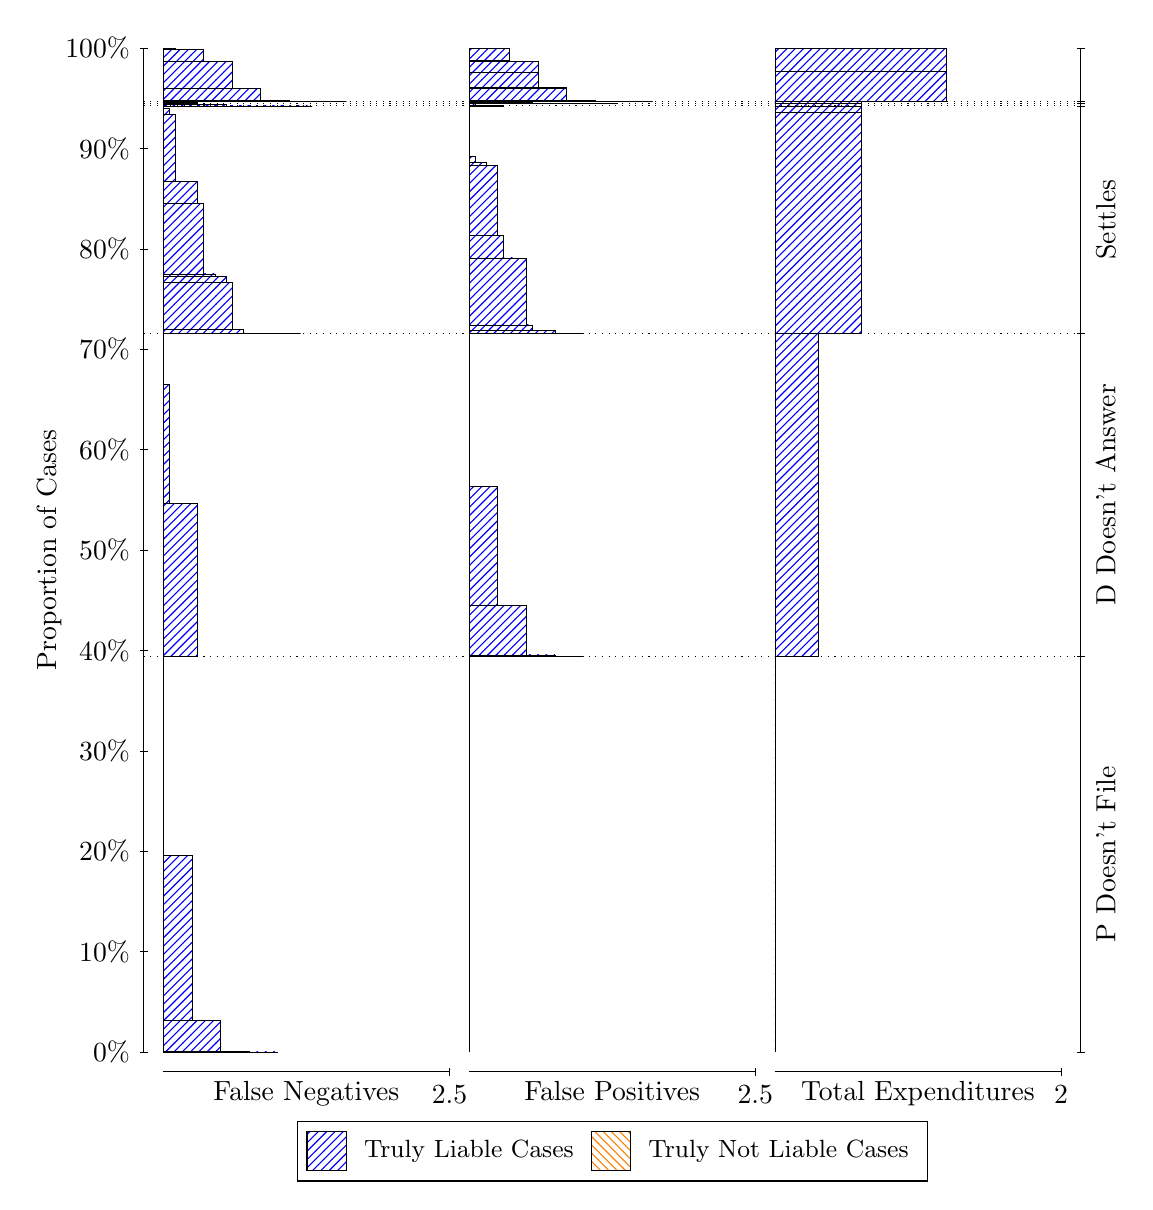
\begin{tikzpicture}
\draw[black, very thin] (1.5,1.75) -- (1.5,14.5);
\node[rotate=90, text=black, anchor=center] at (0.3, 8.125) {Proportion of Cases};
\draw[black, very thin] (1.45,1.75) -- (1.55,1.75);
\node[text=black, anchor=east] at (1.45, 1.75) {0\%};
\draw[black, very thin] (1.45,3.025) -- (1.55,3.025);
\node[text=black, anchor=east] at (1.45, 3.025) {10\%};
\draw[black, very thin] (1.45,4.3) -- (1.55,4.3);
\node[text=black, anchor=east] at (1.45, 4.3) {20\%};
\draw[black, very thin] (1.45,5.575) -- (1.55,5.575);
\node[text=black, anchor=east] at (1.45, 5.575) {30\%};
\draw[black, very thin] (1.45,6.85) -- (1.55,6.85);
\node[text=black, anchor=east] at (1.45, 6.85) {40\%};
\draw[black, very thin] (1.45,8.125) -- (1.55,8.125);
\node[text=black, anchor=east] at (1.45, 8.125) {50\%};
\draw[black, very thin] (1.45,9.4) -- (1.55,9.4);
\node[text=black, anchor=east] at (1.45, 9.4) {60\%};
\draw[black, very thin] (1.45,10.675) -- (1.55,10.675);
\node[text=black, anchor=east] at (1.45, 10.675) {70\%};
\draw[black, very thin] (1.45,11.95) -- (1.55,11.95);
\node[text=black, anchor=east] at (1.45, 11.95) {80\%};
\draw[black, very thin] (1.45,13.225) -- (1.55,13.225);
\node[text=black, anchor=east] at (1.45, 13.225) {90\%};
\draw[black, very thin] (1.45,14.5) -- (1.55,14.5);
\node[text=black, anchor=east] at (1.45, 14.5) {100\%};

\draw[black, very thin] (13.4,1.75) -- (13.4,14.5);
\draw[black, very thin] (13.35,1.75) -- (13.45,1.75);
\node[anchor=west] at (13.35, 1.75) {};
\draw[black, very thin] (13.35,6.7746) -- (13.45,6.7746);
\node[anchor=west] at (13.35, 6.7746) {};
\draw[black, very thin] (13.35,10.877) -- (13.45,10.877);
\node[anchor=west] at (13.35, 10.877) {};
\draw[black, very thin] (13.35,13.765) -- (13.45,13.765);
\node[anchor=west] at (13.35, 13.765) {};
\draw[black, very thin] (13.35,13.796) -- (13.45,13.796);
\node[anchor=west] at (13.35, 13.796) {};
\draw[black, very thin] (13.35,13.825) -- (13.45,13.825);
\node[anchor=west] at (13.35, 13.825) {};
\draw[black, very thin] (13.35,14.5) -- (13.45,14.5);
\node[anchor=west] at (13.35, 14.5) {};

\draw[black, very thin, pattern color=blue, pattern=north east lines] (1.75,1.75) rectangle (3.2033,1.75);
\draw[black, very thin, pattern color=blue, pattern=north east lines] (1.75,1.75) rectangle (2.84,1.7533);
\draw[black, very thin, pattern color=blue, pattern=north east lines] (1.75,1.7533) rectangle (2.4767,2.1466);
\draw[black, very thin, pattern color=blue, pattern=north east lines] (1.75,2.1466) rectangle (2.1133,4.2421);
\draw[black, very thin, pattern color=orange, pattern=north west lines] (1.75,4.2421) rectangle (1.75,4.2421);
\draw[black, very thin, pattern color=blue, pattern=north east lines] (1.75,4.2421) rectangle (1.75,6.7746);
\draw[black, very thin, pattern color=blue, pattern=north east lines] (1.75,6.7746) rectangle (2.186,8.7142);
\draw[black, very thin, pattern color=blue, pattern=north east lines] (1.75,8.7142) rectangle (1.8227,10.231);
\draw[black, very thin, pattern color=orange, pattern=north west lines] (1.75,10.231) rectangle (1.75,10.231);
\draw[black, very thin, pattern color=blue, pattern=north east lines] (1.75,10.231) rectangle (1.75,10.877);
\draw[black, very thin, pattern color=blue, pattern=north east lines] (1.75,10.877) rectangle (3.494,10.877);
\draw[black, very thin, pattern color=blue, pattern=north east lines] (1.75,10.877) rectangle (3.1307,10.878);
\draw[black, very thin, pattern color=blue, pattern=north east lines] (1.75,10.878) rectangle (2.9127,10.88);
\draw[black, very thin, pattern color=blue, pattern=north east lines] (1.75,10.88) rectangle (2.7673,10.926);
\draw[black, very thin, pattern color=blue, pattern=north east lines] (1.75,10.926) rectangle (2.622,11.522);
\draw[black, very thin, pattern color=blue, pattern=north east lines] (1.75,11.522) rectangle (2.5493,11.598);
\draw[black, very thin, pattern color=blue, pattern=north east lines] (1.75,11.598) rectangle (2.404,11.633);
\draw[black, very thin, pattern color=blue, pattern=north east lines] (1.75,11.633) rectangle (2.2587,12.523);
\draw[black, very thin, pattern color=blue, pattern=north east lines] (1.75,12.523) rectangle (2.186,12.808);
\draw[black, very thin, pattern color=blue, pattern=north east lines] (1.75,12.808) rectangle (2.0407,12.808);
\draw[black, very thin, pattern color=blue, pattern=north east lines] (1.75,12.808) rectangle (1.8953,13.659);
\draw[black, very thin, pattern color=blue, pattern=north east lines] (1.75,13.659) rectangle (1.8227,13.731);
\draw[black, very thin, pattern color=orange, pattern=north west lines] (1.75,13.731) rectangle (1.75,13.731);
\draw[black, very thin, pattern color=blue, pattern=north east lines] (1.75,13.731) rectangle (1.75,13.765);
\draw[black, very thin, pattern color=blue, pattern=north east lines] (1.75,13.765) rectangle (3.6393,13.765);
\draw[black, very thin, pattern color=blue, pattern=north east lines] (1.75,13.765) rectangle (3.276,13.765);
\draw[black, very thin, pattern color=blue, pattern=north east lines] (1.75,13.765) rectangle (2.9127,13.765);
\draw[black, very thin, pattern color=blue, pattern=north east lines] (1.75,13.765) rectangle (2.5493,13.784);
\draw[black, very thin, pattern color=blue, pattern=north east lines] (1.75,13.784) rectangle (2.186,13.796);
\draw[black, very thin, pattern color=orange, pattern=north west lines] (1.75,13.796) rectangle (1.75,13.796);
\draw[black, very thin, pattern color=blue, pattern=north east lines] (1.75,13.796) rectangle (2.186,13.807);
\draw[black, very thin, pattern color=blue, pattern=north east lines] (1.75,13.807) rectangle (1.8227,13.824);
\draw[black, very thin, pattern color=orange, pattern=north west lines] (1.75,13.824) rectangle (1.75,13.824);
\draw[black, very thin, pattern color=blue, pattern=north east lines] (1.75,13.824) rectangle (1.75,13.825);
\draw[black, very thin, pattern color=blue, pattern=north east lines] (1.75,13.825) rectangle (4.0753,13.825);
\draw[black, very thin, pattern color=blue, pattern=north east lines] (1.75,13.825) rectangle (3.712,13.825);
\draw[black, very thin, pattern color=blue, pattern=north east lines] (1.75,13.825) rectangle (3.3487,13.834);
\draw[black, very thin, pattern color=blue, pattern=north east lines] (1.75,13.834) rectangle (2.9853,13.99);
\draw[black, very thin, pattern color=blue, pattern=north east lines] (1.75,13.99) rectangle (2.622,14.329);
\draw[black, very thin, pattern color=blue, pattern=north east lines] (1.75,14.329) rectangle (2.2587,14.486);
\draw[black, very thin, pattern color=blue, pattern=north east lines] (1.75,14.486) rectangle (1.8953,14.5);
\draw[black, very thin, pattern color=orange, pattern=north west lines] (1.75,14.5) rectangle (1.75,14.5);
\draw[black, very thin, pattern color=blue, pattern=north east lines] (1.75,14.5) rectangle (1.75,14.5);
\draw[black, very thin, pattern color=orange, pattern=north west lines] (5.6333,1.75) rectangle (5.6333,1.75);
\draw[black, very thin, pattern color=blue, pattern=north east lines] (5.6333,1.75) rectangle (5.6333,6.7746);
\draw[black, very thin, pattern color=orange, pattern=north west lines] (5.6333,6.7746) rectangle (7.0867,6.7746);
\draw[black, very thin, pattern color=blue, pattern=north east lines] (5.6333,6.7746) rectangle (7.0867,6.7746);
\draw[black, very thin, pattern color=blue, pattern=north east lines] (5.6333,6.7746) rectangle (6.7233,6.793);
\draw[black, very thin, pattern color=blue, pattern=north east lines] (5.6333,6.793) rectangle (6.36,7.4206);
\draw[black, very thin, pattern color=blue, pattern=north east lines] (5.6333,7.4206) rectangle (5.9967,8.9375);
\draw[black, very thin, pattern color=blue, pattern=north east lines] (5.6333,8.9375) rectangle (5.6333,10.877);
\draw[black, very thin, pattern color=orange, pattern=north west lines] (5.6333,10.877) rectangle (7.0867,10.877);
\draw[black, very thin, pattern color=blue, pattern=north east lines] (5.6333,10.877) rectangle (7.0867,10.877);
\draw[black, very thin, pattern color=orange, pattern=north west lines] (5.6333,10.877) rectangle (6.796,10.877);
\draw[black, very thin, pattern color=blue, pattern=north east lines] (5.6333,10.877) rectangle (6.796,10.879);
\draw[black, very thin, pattern color=blue, pattern=north east lines] (5.6333,10.879) rectangle (6.7233,10.911);
\draw[black, very thin, pattern color=blue, pattern=north east lines] (5.6333,10.911) rectangle (6.4327,10.983);
\draw[black, very thin, pattern color=blue, pattern=north east lines] (5.6333,10.983) rectangle (6.36,11.833);
\draw[black, very thin, pattern color=orange, pattern=north west lines] (5.6333,11.833) rectangle (6.2147,11.833);
\draw[black, very thin, pattern color=blue, pattern=north east lines] (5.6333,11.833) rectangle (6.2147,11.834);
\draw[black, very thin, pattern color=blue, pattern=north east lines] (5.6333,11.834) rectangle (6.0693,12.119);
\draw[black, very thin, pattern color=blue, pattern=north east lines] (5.6333,12.119) rectangle (5.9967,13.009);
\draw[black, very thin, pattern color=blue, pattern=north east lines] (5.6333,13.009) rectangle (5.8513,13.044);
\draw[black, very thin, pattern color=blue, pattern=north east lines] (5.6333,13.044) rectangle (5.706,13.12);
\draw[black, very thin, pattern color=blue, pattern=north east lines] (5.6333,13.12) rectangle (5.6333,13.765);
\draw[black, very thin, pattern color=orange, pattern=north west lines] (5.6333,13.765) rectangle (6.0693,13.765);
\draw[black, very thin, pattern color=blue, pattern=north east lines] (5.6333,13.765) rectangle (6.0693,13.776);
\draw[black, very thin, pattern color=blue, pattern=north east lines] (5.6333,13.776) rectangle (5.706,13.795);
\draw[black, very thin, pattern color=blue, pattern=north east lines] (5.6333,13.795) rectangle (5.6333,13.796);
\draw[black, very thin, pattern color=orange, pattern=north west lines] (5.6333,13.796) rectangle (7.5227,13.796);
\draw[black, very thin, pattern color=blue, pattern=north east lines] (5.6333,13.796) rectangle (7.5227,13.796);
\draw[black, very thin, pattern color=blue, pattern=north east lines] (5.6333,13.796) rectangle (7.1593,13.796);
\draw[black, very thin, pattern color=blue, pattern=north east lines] (5.6333,13.796) rectangle (6.796,13.796);
\draw[black, very thin, pattern color=blue, pattern=north east lines] (5.6333,13.796) rectangle (6.4327,13.813);
\draw[black, very thin, pattern color=blue, pattern=north east lines] (5.6333,13.813) rectangle (6.0693,13.825);
\draw[black, very thin, pattern color=orange, pattern=north west lines] (5.6333,13.825) rectangle (7.9587,13.825);
\draw[black, very thin, pattern color=blue, pattern=north east lines] (5.6333,13.825) rectangle (7.9587,13.825);
\draw[black, very thin, pattern color=orange, pattern=north west lines] (5.6333,13.825) rectangle (7.5953,13.825);
\draw[black, very thin, pattern color=blue, pattern=north east lines] (5.6333,13.825) rectangle (7.5953,13.825);
\draw[black, very thin, pattern color=orange, pattern=north west lines] (5.6333,13.825) rectangle (7.232,13.825);
\draw[black, very thin, pattern color=blue, pattern=north east lines] (5.6333,13.825) rectangle (7.232,13.839);
\draw[black, very thin, pattern color=blue, pattern=north east lines] (5.6333,13.839) rectangle (6.8687,13.995);
\draw[black, very thin, pattern color=orange, pattern=north west lines] (5.6333,13.995) rectangle (6.8687,13.995);
\draw[black, very thin, pattern color=blue, pattern=north east lines] (5.6333,13.995) rectangle (6.8687,13.996);
\draw[black, very thin, pattern color=blue, pattern=north east lines] (5.6333,13.996) rectangle (6.5053,14.191);
\draw[black, very thin, pattern color=orange, pattern=north west lines] (5.6333,14.191) rectangle (6.5053,14.191);
\draw[black, very thin, pattern color=blue, pattern=north east lines] (5.6333,14.191) rectangle (6.5053,14.335);
\draw[black, very thin, pattern color=blue, pattern=north east lines] (5.6333,14.335) rectangle (6.142,14.346);
\draw[black, very thin, pattern color=blue, pattern=north east lines] (5.6333,14.346) rectangle (6.142,14.491);
\draw[black, very thin, pattern color=blue, pattern=north east lines] (5.6333,14.491) rectangle (5.7787,14.491);
\draw[black, very thin, pattern color=blue, pattern=north east lines] (5.6333,14.491) rectangle (5.7787,14.5);
\draw[black, very thin, pattern color=blue, pattern=north east lines] (5.6333,14.5) rectangle (5.6333,14.5);
\draw[black, very thin, pattern color=orange, pattern=north west lines] (9.5167,1.75) rectangle (9.5167,1.75);
\draw[black, very thin, pattern color=blue, pattern=north east lines] (9.5167,1.75) rectangle (9.5167,6.7746);
\draw[black, very thin, pattern color=orange, pattern=north west lines] (9.5167,6.7746) rectangle (10.062,6.7746);
\draw[black, very thin, pattern color=blue, pattern=north east lines] (9.5167,6.7746) rectangle (10.062,10.877);
\draw[black, very thin, pattern color=orange, pattern=north west lines] (9.5167,10.877) rectangle (10.607,10.877);
\draw[black, very thin, pattern color=blue, pattern=north east lines] (9.5167,10.877) rectangle (10.607,13.683);
\draw[black, very thin, pattern color=orange, pattern=north west lines] (9.5167,13.683) rectangle (10.607,13.683);
\draw[black, very thin, pattern color=blue, pattern=north east lines] (9.5167,13.683) rectangle (10.607,13.765);
\draw[black, very thin, pattern color=orange, pattern=north west lines] (9.5167,13.765) rectangle (10.607,13.765);
\draw[black, very thin, pattern color=blue, pattern=north east lines] (9.5167,13.765) rectangle (10.607,13.796);
\draw[black, very thin, pattern color=orange, pattern=north west lines] (9.5167,13.796) rectangle (10.607,13.796);
\draw[black, very thin, pattern color=blue, pattern=north east lines] (9.5167,13.796) rectangle (10.607,13.825);
\draw[black, very thin, pattern color=orange, pattern=north west lines] (9.5167,13.825) rectangle (11.697,13.825);
\draw[black, very thin, pattern color=blue, pattern=north east lines] (9.5167,13.825) rectangle (11.697,14.201);
\draw[black, very thin, pattern color=orange, pattern=north west lines] (9.5167,14.201) rectangle (11.697,14.201);
\draw[black, very thin, pattern color=blue, pattern=north east lines] (9.5167,14.201) rectangle (11.697,14.5);
\draw[black, dotted] (1.5,6.7746) -- (13.4,6.7746);
\draw[black, dotted] (1.5,10.877) -- (13.4,10.877);
\draw[black, dotted] (1.5,13.765) -- (13.4,13.765);
\draw[black, dotted] (1.5,13.796) -- (13.4,13.796);
\draw[black, dotted] (1.5,13.825) -- (13.4,13.825);
\draw[black, very thin] (1.75,1.5) -- (5.3833,1.5);
\node[text=black, anchor=north] at (3.5667, 1.5) {False Negatives};
\draw[black, very thin] (5.3833,1.45) -- (5.3833,1.55);
\node[text=black, anchor=north] at (5.3833, 1.45) {2.5};

\draw[black, very thin] (5.6333,1.5) -- (9.2667,1.5);
\node[text=black, anchor=north] at (7.45, 1.5) {False Positives};
\draw[black, very thin] (9.2667,1.45) -- (9.2667,1.55);
\node[text=black, anchor=north] at (9.2667, 1.45) {2.5};

\draw[black, very thin] (9.5167,1.5) -- (13.15,1.5);
\node[text=black, anchor=north] at (11.333, 1.5) {Total Expenditures};
\draw[black, very thin] (13.15,1.45) -- (13.15,1.55);
\node[text=black, anchor=north] at (13.15, 1.45) {2};

\node[text=black, centered, rotate=90] at (13.72, 4.2623) {P Doesn't File};
\node[text=black, centered, rotate=90] at (13.72, 8.8258) {D Doesn't Answer};
\node[text=black, centered, rotate=90] at (13.72, 12.321) {Settles};




\draw (7.449999999999999,1.5) node[draw=none] (baseCoordinate) {};
\begin{scope}[align=center]
        \matrix[scale=0.5, draw=black, below=0.5cm of baseCoordinate, nodes={draw}, column sep=0.1cm]{
            \node[rectangle, draw, minimum width=0.5cm, minimum height=0.5cm, pattern color=blue, pattern=north east lines] {}; &
            \node[draw=none, font=\small, text=black] (B) {Truly Liable Cases}; &
            \node[rectangle, draw, minimum width=0.5cm, minimum height=0.5cm, pattern color=orange, pattern=north west lines] {}; &
            \node[draw=none, font=\small, text=black] (B) {Truly Not Liable Cases}; \\
            };
\end{scope}

\end{tikzpicture}
\end{document}